\section{Généralités sur le cerveau}

Pour mieux comprendre l'aphasie en général et celle de Broca en particulier, 
il convient de commencer avec le cerveau.
Il s'agit du système biologique le plus complexe connu~\cite{}.
Avec le cervelet et le tronc cérébral, il forme l'encéphale (voir Figure~\ref{fig:brain}).
Le cerveau se charge du traitement des flux nerveux sensoriels et moteurs.
Il est aussi le siège des hautes fonctions cognitives comme l'inférence logique, l'émotion 
et --- crucialement pour notre étude --- le traitement du langage~\cite{}.

\begin{figure}[htb]
    \begin{center}
        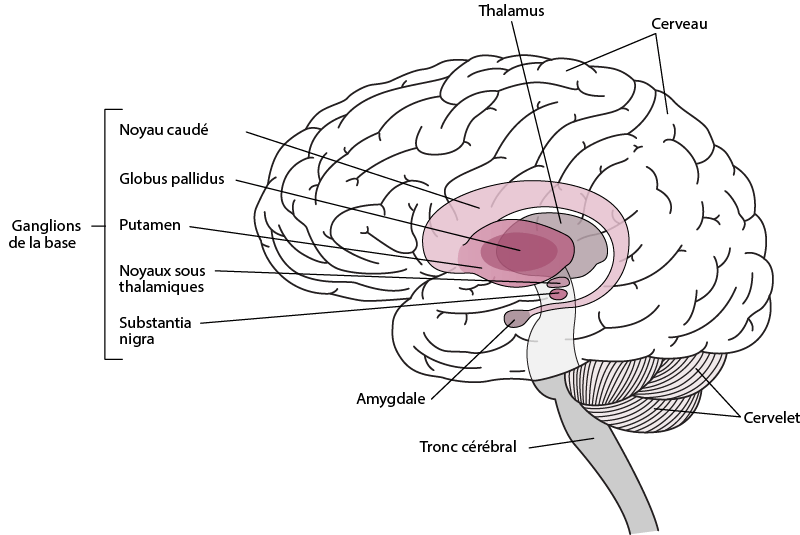
\includegraphics[width=.8\textwidth]{brain.png}
    \end{center}
    \caption{Encéphale humain}
    \label{fig:brain}
\end{figure}

Le cerveau est composé de deux hémisphères ; chacun desquels se divise en lobes : 
frontal, temporal, pariétal et occipital (voir Figure~\ref{fig:lobes}).
La surface du cerveau s'appelle le ``cortex cérébral''.
Il présente plusieurs circonvolutions qui augmentent considérablement sa surface.
Le cortex cérébral est divisé en régions fonctionnelles que nous appelons ``aires''
(voir Figure~\ref{fig:brain-areas}).
Le travail de Dr.~Broca sur le cas de M.~Leborgne est largement reconnu comme l'origine de cette division.


\begin{figure}[htb]
    \begin{center}
        \subfloat[Lobes du cerveau~\cite{}]{
            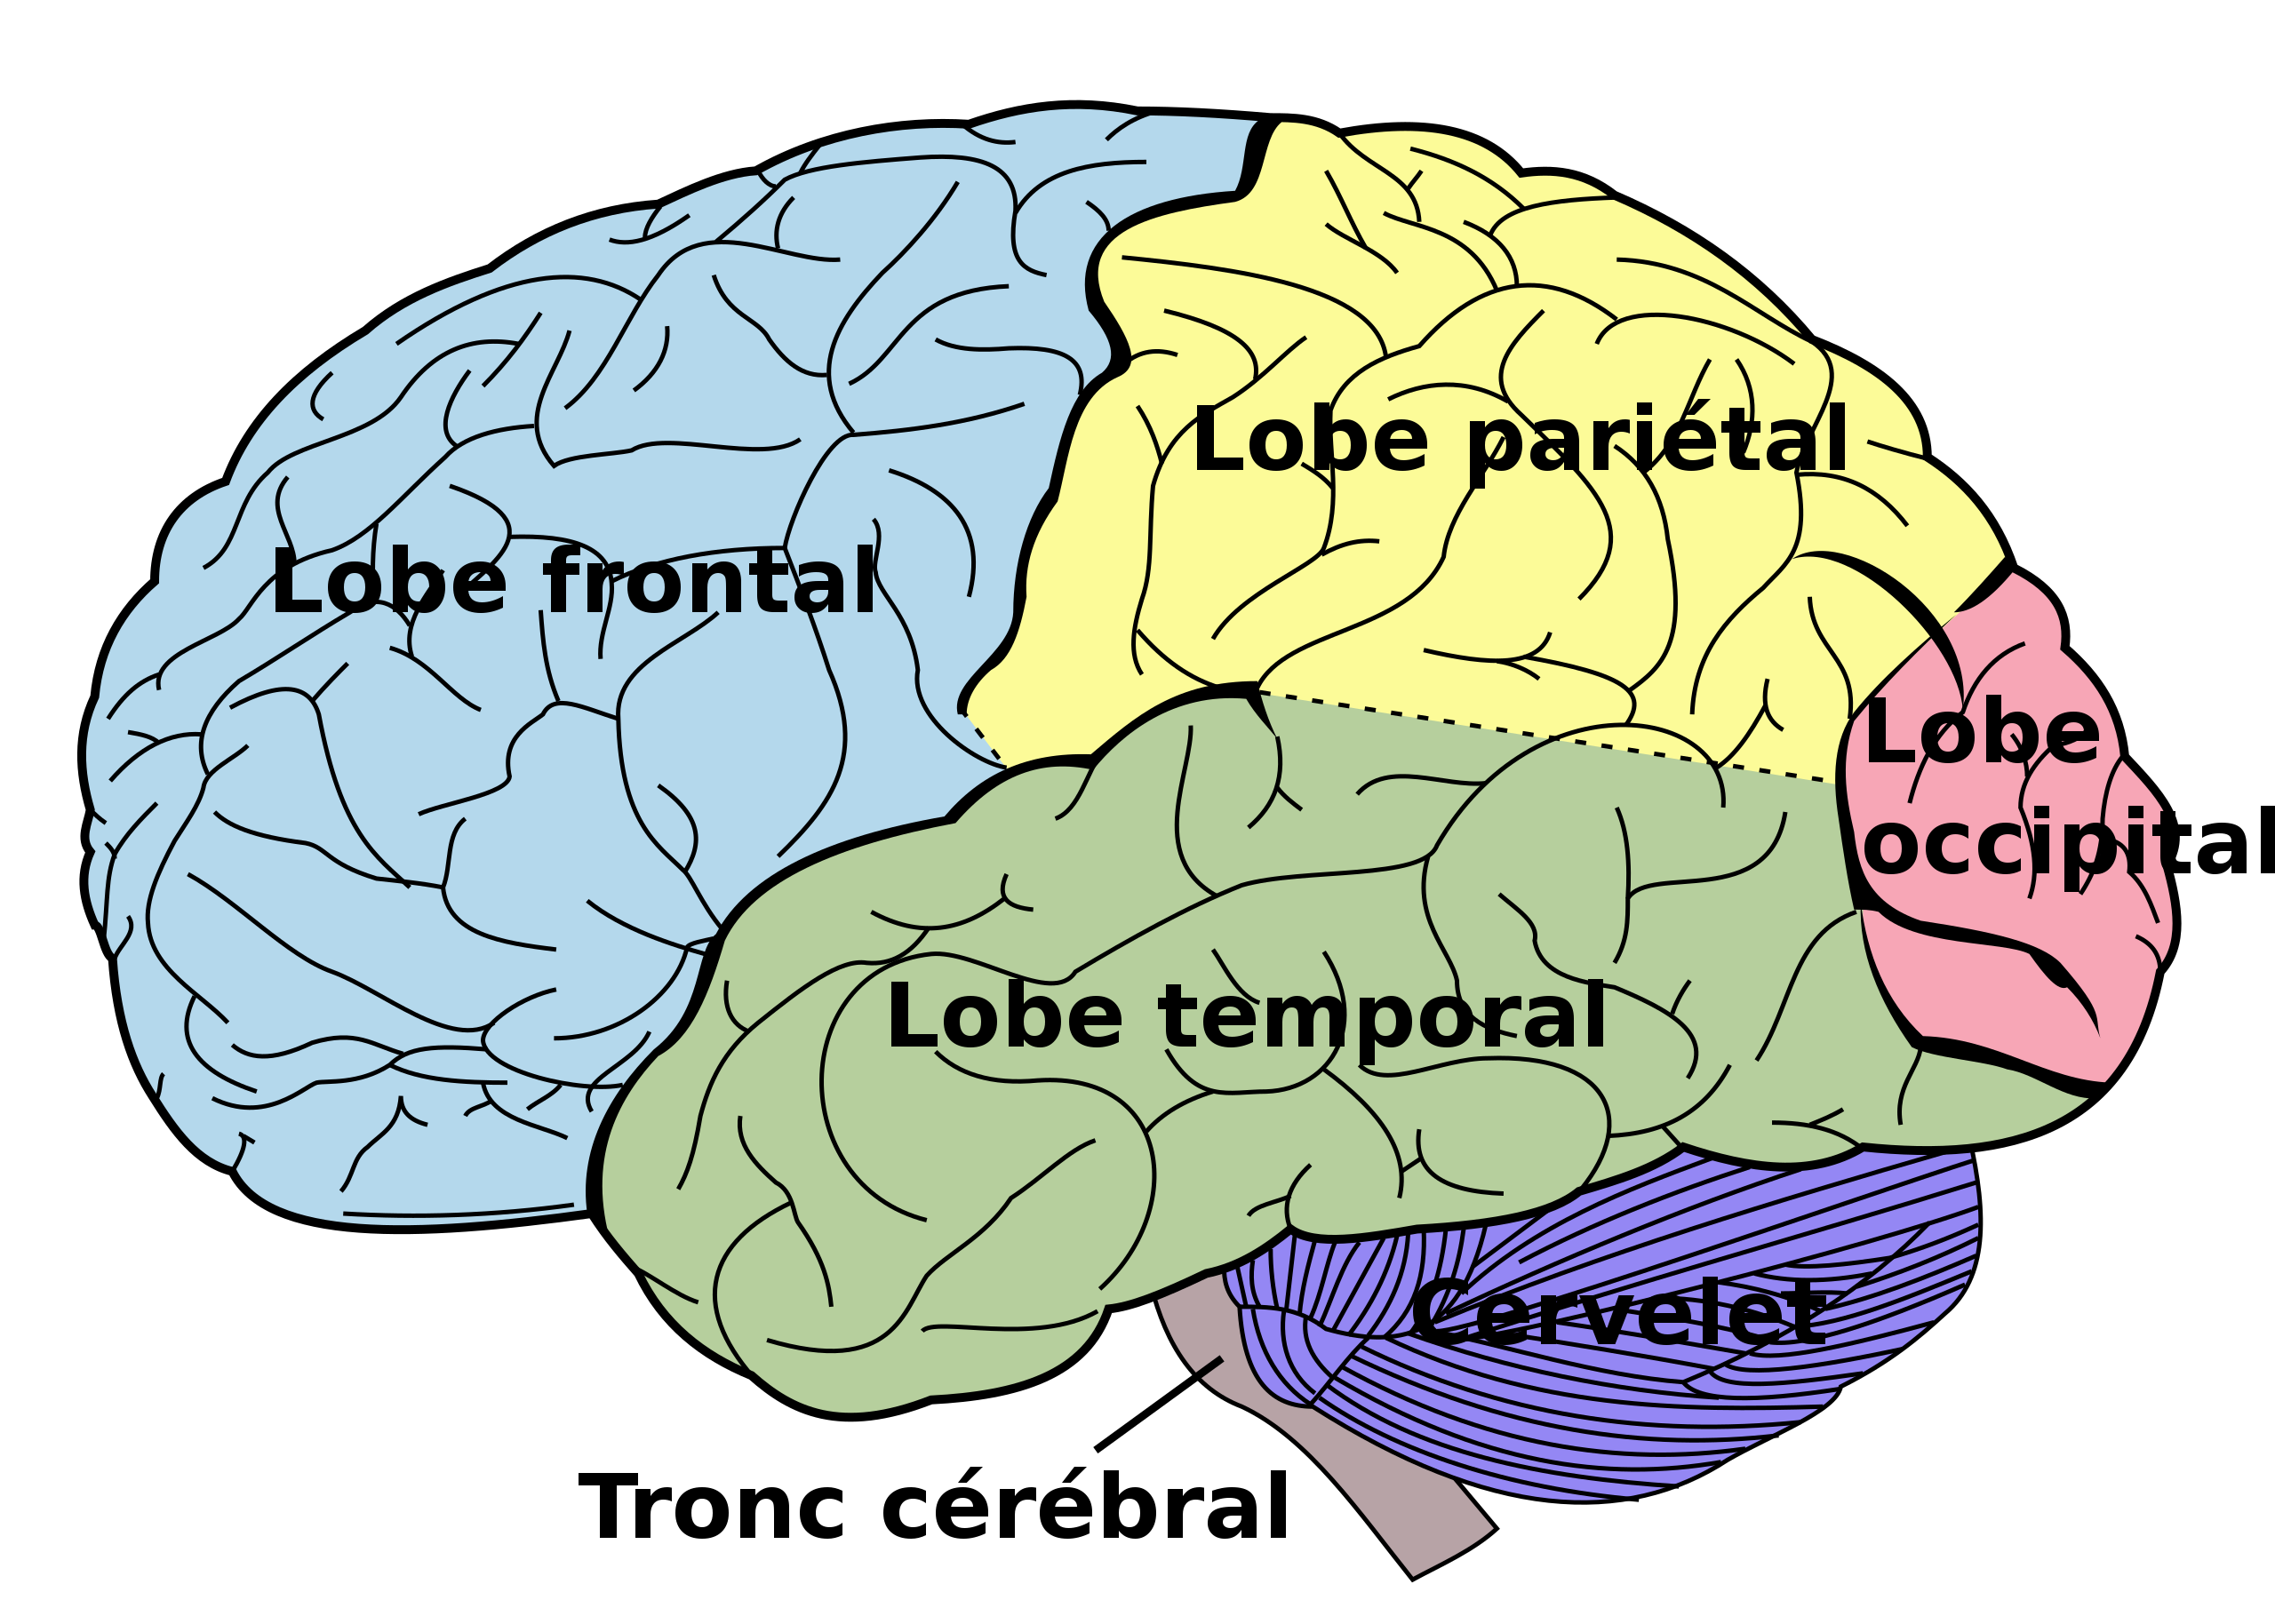
\includegraphics[width=.45\textwidth]{lobes.png}
            \label{fig:lobes}
        }
        \subfloat[Aires du cortex cérébral~\cite{}]{
            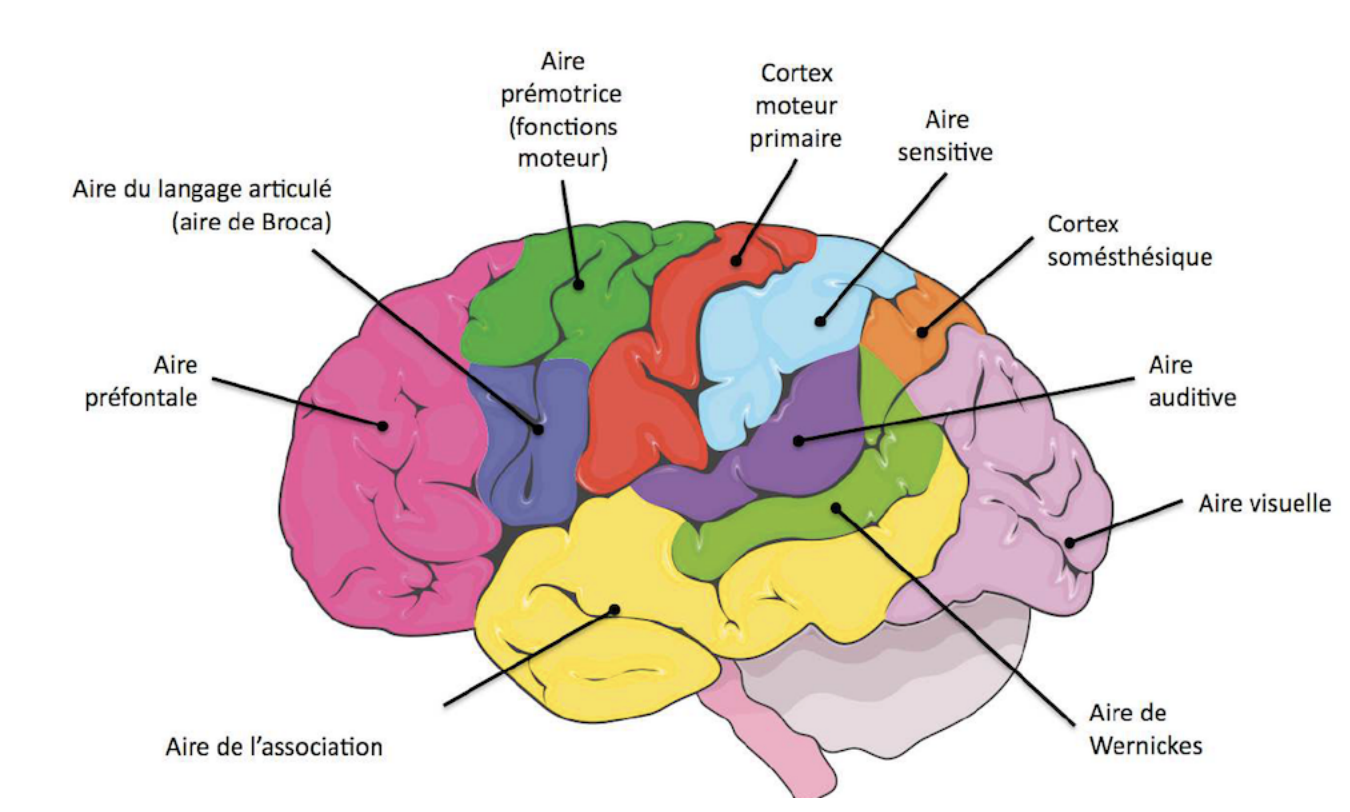
\includegraphics[width=.45\textwidth]{areas.png}
            \label{fig:brain-areas}
        }
    \end{center}
    \caption{Division morphologique et fonctionnelle du cerveau.}
\end{figure}

Une autre division importante et due à l'anatomiste Allemand Korbinian Brodmann.
Elle se base sur l'organisation cellulaire des neurones pour segmenter le cortex cérébral en 52 régions 
aussi nommées ``aires''.
En dépit d'avoir une définition morphologique, 
les aires de Brodmann sont largement alignés sur les aires fonctionnelles 
de la Figure~\ref{fig:brain-areas}~\cite{Brodmann_2007}.

